\part[Concurrency]{Concurrency}
\section{The World of Computing Today}
\begin{frame}{Moore's Law}
\begin{center}
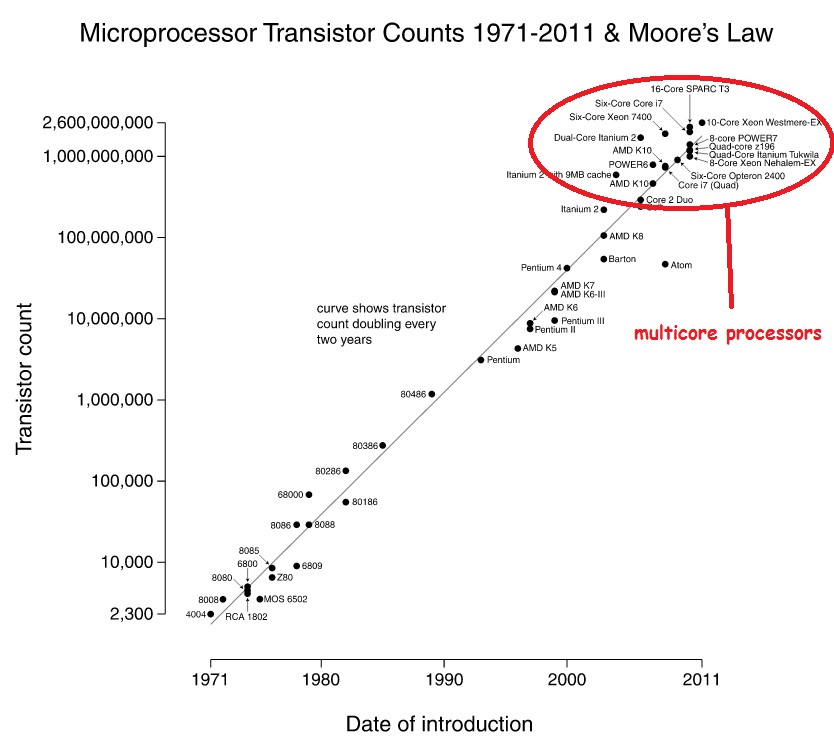
\includegraphics[width = 0.8\textwidth]{resources/Moores-Law.jpg}
\end{center}
\end{frame}

\begin{frame}{When the hardware changes, software follows\ldots}
\begin{block}{Concurrency tools today}
\begin{itemize}
  \item \sout{Threads and locks}
  \item Actors with messages
  \item Agents
  \item Software Transaction Memory (STM)
\end{itemize}
\end{block}
\begin{block}{Popular Parallel Programming Challenge (PPP)}
\begin{itemize}
  \item Fundamental problem: \highlight{non-determinism}
  \item Leads to \highlight{Heisenbugs}, different behavior on different
  hardware
\end{itemize}
\end{block}
\end{frame}

\begin{frame}{Heisenbug}
\emph{``[from Heisenberg's Uncertainty Principle in quantum physics] A bug that
disappears or \alert{alters} its \alert{behavior when} one attempts to
\alert{probe} or isolate it. (This usage is not even particularly fanciful; the
use of a debugger sometimes alters a program's operating environment significantly enough that buggy code,
such as that which relies on the values of uninitialized memory, behaves quite
differently.) Antonym of Bohr bug; see also mandelbug, schroedinbug. In
\alert{C}, nine out of ten heisenbugs result from uninitialized auto variables,
fandango on core phenomena (esp. lossage related to corruption of the malloc
arena) or errors that smash the stack.''} -
\link{www.definitions.net}{www.definitions.net}
\end{frame}


\begin{frame}[fragile]{The Root of the Problem}
\begin{alertblock}{Problem}
\begin{itemize}
  \item Non-determinism caused by concurrent threads accessing \alert{shared
  mutable state}
  \item We can encapsulate state in actors or transactions, but the fundamental
  problem is the same
\end{itemize}
\begin{center}
non-determinism = parallel processing + \alert{mutable state}
\end{center}
\end{alertblock}
\begin{center}
\lstinline!var x = 0!\\
\lstinline!async { x = x + 1 }!\\
\lstinline!async { x = x * 2 }!\\
\lstinline!// x can give 0, 1, 2!\\
\end{center}
\begin{exampleblock}{Solution}
\begin{itemize}
  \item To get deterministic processing, \alert{avoid} the mutable state!
  \item Avoiding mutable state means programming \highlight{functionally}
\end{itemize}
\end{exampleblock}
\end{frame}

\begin{frame}[fragile]{Functional Programming to the rescue}
\begin{block}{What is FP all about?}
FP is about \highlight{transforming the data} instead of changing data in place.
You pipe the data from one point to another through a bunch of transformers
without changing the original, without changing the intermediates and you get
what you wanted. This \highlight{scales} and this is \highlight{threadsafe}. All
we need are tools to make it happen \highlight{concurrently}\ldots
\end{block}

\begin{exampleblock}{What is FP all about?}
\begin{lstlisting}
scala> Vector("1", "2", "3", "4")
     |   .map { _.toInt }
     |   .filter { _ % 2 == 0 }
     |   .sum
res0: Int = 6
\end{lstlisting}
\end{exampleblock}
\end{frame}

\section{Akka}
\begin{frame}{Akka}
\begin{block}{What is Akka?}
Akka is a \highlight{toolkit} and runtime for building highly concurrent,
distributed, and fault tolerant event-driven applications on the JVM.
\end{block}
\pause
\begin{block}{What is in the toolkit?}
\highlight{Actors}, typed actors, logging, event bus, scheduler,
\highlight{futures}, dataflow concurrency, fault tolerance, dispatchers,
routing, remoting, serialization, FSM, STM, Agents, Transactors, IO, Testkit,
MicroKernel, ZeroMQ
\end{block}
\end{frame}

\begin{frame}[fragile]{Akka}
\begin{block}{5 Concurrency Options (ordered by increasing complexity \& overhead)}
\begin{enumerate}
  \item \lstinline!java.util.concurrent! (Akka is built on top of j.u.c)
  \item Scala parallel collections
  \item Akka/Scala Futures
  \item Akka/Scala Dataflow (not accessible from Java)
  \item Akka/Scala Actors
\end{enumerate}
\end{block}
\pause
\begin{block}{Reminder j.u.c primitives}
\begin{itemize}
  \item \lstinline!Callable!, \lstinline!Runnable!
  \item \lstinline!Thread!s, thread pools and \lstinline!Executor!s
  \item \lstinline!CompletionService!, \lstinline!CountDownLatch!, concurrent
  collections, \lstinline!CyclicBarrier!, \lstinline!Phaser!,
  \lstinline!Semaphore!, \lstinline!TimeUnit!
  \item Primitive \lstinline!Future<T>!
\end{itemize}
\end{block}
\end{frame}

\begin{frame}{Akka Dispatchers and j.u.c}
\begin{center}
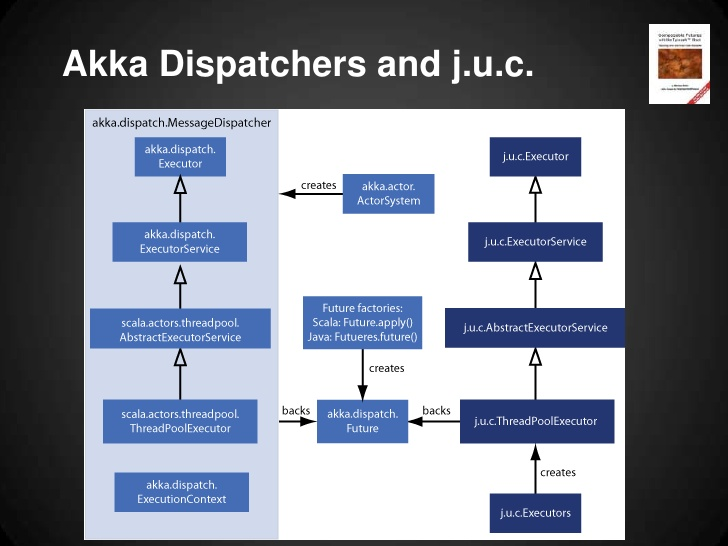
\includegraphics[width = 0.8\textwidth]{resources/JUC.jpg}
\end{center}
\end{frame}

\subsection{Futures and Promises}
\begin{frame}{Futures and Promises}
\begin{block}{What is a Future?}
A \highlight{Future} is a \highlight{read-handle} to a single value
\highlight{(read-many)} that \highlight{may} be available within a specific
time-frame.
\end{block}
\pause
\begin{block}{What is a Promise?}
A \highlight{Promise} is a \highlight{write-handle} to a single value
\highlight{(write-once)} that \highlight{should} be made available within a
specific time-frame.
\end{block}
\end{frame}

\begin{frame}[fragile]{Futures}
\begin{block}{Creating futures (with Scala 2.10)}
\begin{lstlisting}
// Definition
def future[T](body: => T)
  (implicit ec: ExecutionContext = defaultExecutionContext): Future[T]
    
// Usage
import scala.concurrent.future
val friends: Future[Set[Profiles]] = future { profile.getFriends }
\end{lstlisting}
\end{block}
\pause
\begin{block}{The Hollywood Principle}
\begin{lstlisting}
class Future[+T] {
  def onComplete[U](f: Either[Throwable, T] => U): this.type
}
\end{lstlisting}
\end{block}
\end{frame}

\begin{frame}[fragile]{Futures are monads}
\begin{exampleblock}{Remember these?}
\begin{lstlisting}
class List[+A] {
  def foreach[B](f: A => B): Unit
  def map[B](f: A => B): List[B]
  def flatMap[B](f: A => List[B]): List[B]
  def filter(p: A => Boolean): List[A]
}
\end{lstlisting}
\end{exampleblock}
\pause
\begin{exampleblock}{How about those?}
\begin{lstlisting}
class Future[+A] {
  def foreach[B](f: A => B): Unit
  def map[B](f: A => B): Future[B]
  def flatMap[B](f: A => Future[B]): Future[B]
  def filter(p: A => Boolean): Future[A]
}
\end{lstlisting}
\end{exampleblock}
\end{frame}

\begin{frame}[fragile]{Futures are monads}
\begin{exampleblock}{Monads are all about composability}
\begin{lstlisting}
def sum(f1: Future[Int], f2: Future[Int]): Future[Int] = for {
   v1 <- f1
   v2 <- f2
} yield v1 + v2
\end{lstlisting}
\end{exampleblock}
\pause
\begin{exampleblock}{Futures are asynchronous}
\begin{lstlisting}
scala> val f3 = sum(future { Thread.sleep(5000); 1 }, future { 2 })
f3: Future[Int] = ...

scala> f3 foreach println
3 // when the time comes
\end{lstlisting}
\end{exampleblock}
\end{frame}

\begin{frame}[fragile]{Future API}
\begin{block}{\lstinline!collect!}
\lstinline!def collect[S](pf: PartialFunction[T, S]): Future[S]!
\end{block}
\begin{exampleblock}{\lstinline!collect!}
\lstinline!val f2 = f collect { case Identifier(x) => camelCase(x) }!
\end{exampleblock}
\pause
\begin{block}{\lstinline!recover!}
\lstinline!def recover[U >: T](pf: PartialFunction[Throwable, U]): Future[U]!
\end{block}
\begin{exampleblock}{\lstinline!recover!}
\begin{lstlisting}
val f = future { 1 / 0 } recover {
  case a: ArithmeticException => 0
}
\end{lstlisting}
\end{exampleblock}
\end{frame}

\begin{frame}[fragile]{Future API}
\begin{block}{\lstinline!fallbackTo!}
\lstinline!def fallbackTo[U >: T](that: Future[U]): Future[U]!
\end{block}
\begin{exampleblock}{\lstinline!fallbackTo!}
\begin{lstlisting}
val image = future { loadimageFromInterwebz() }
val result = image fallbackTo pictureOfKittens
\end{lstlisting}
\end{exampleblock}
\pause
\begin{block}{\lstinline!either!}
\lstinline!def either[U >: T](that: Future[U]): Future[U]!
\end{block}
\begin{exampleblock}{\lstinline!either!}
\begin{lstlisting}
val f1 = future { loadImageFrom(node1) }
val f2 = future { loadImageFrom(node2) }
val result = f1 either f2
\end{lstlisting}
\end{exampleblock}
\end{frame}

\begin{frame}[fragile]{Promises}
\begin{block}{Creating promises (with Scala 2.10)}
\begin{lstlisting}
// Definition
def promise[T]()
  (implicit ec: ExecutionContext = defaultExecutionContext): Promise[T]
    
// Usage
import scala.concurrent.promise
val myPromise = promise[BetterWorld]()
\end{lstlisting}
\end{block}
\end{frame}

\begin{frame}[fragile]{Promises}
\begin{exampleblock}{Using promises}
\begin{lstlisting}
scala> val p = promise[Int]()
p: Promise[Int] = ...

scala> p success 4711
res0: p.type = ... 

scala> val f = p.future
f: Future[Int]

scala> f foreach println
4711
\end{lstlisting}
\end{exampleblock}
\end{frame}

\begin{frame}{Further Readings}
\begin{center}
\link{http://www.infoq.com/interviews/klang-akka}{Viktor Klang (Akka CTO) on
Akka, Futures and Promises (Video)}
\end{center}
\begin{center}
\link{http://skillsmatter.com/podcast/agile-testing/the-future-i-was-promised}{Viktor
Klang (Akka CTO) - The Future I was Promised (Video)}
\end{center}
\begin{center}
\link{http://www.youtube.com/watch?v=VCattsfHR4o}{Mike Slinn - Composable
Futures with Akka 2.0 (Video)}
\end{center}
\end{frame}

\subsection{Actors}
\begin{frame}{The Actor Model of Computation}
\begin{center}
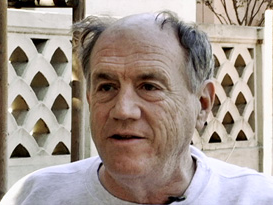
\includegraphics{resources/CarlHewitt.png}
\end{center}
\end{frame}

\begin{frame}{The Actor Model of Computation}
\begin{block}{What is the Actor model?}
\emph{``The Actor model is a \highlight{mathematical theory} that treats
``Actors'' as the \highlight{universal primitives of concurrent digital
computation}. The model has been used both as a framework for a theoretical
understanding of concurrency, and as the theoretical basis for several practical
implementations of concurrent systems. Unlike previous models of computation,
the Actor model was inspired by \highlight{physical laws}. It was also
influenced by the programming languages Lisp, Simula 67 and Smalltalk-72, as
well as ideas for Petri Nets, capability-based systems and packet switching. The
advent of massive concurrency through client-cloud computing and many-core
computer architectures has galvanized interest in the Actor model.''} - Carl Hewitt
\end{block}
\end{frame}

\begin{frame}{The Actor Model of Computation}
\begin{block}{What is an Actor?}
The Actor is the \highlight{fundamental unit of computation}. As the fundamental
unit of computation it has to embody three things:
\begin{enumerate}
  \item Processing
  \item Storage
  \item Communication
\end{enumerate}
\end{block}
\pause
\begin{center}
One Actor is ``not'' an Actor. Actors come in systems.
\end{center}
\begin{block}{What can an actor do?}
In response to a message the Actor receives, it can:
\begin{itemize}
  \item send messages to other Actors
  \item create new Actors
  \item designate how to handle the next message it receives
\end{itemize}
\end{block}
\end{frame}

\begin{frame}{The Actor Model of Computation}
\begin{block}{Actors are purely asynchronous}
\begin{itemize}
  \item When an actor receives a message it \highlight{does not block}
  \item When an actor sends a message it \highlight{does not block}
  \item When an actor processes a message his \highlight{mailbox is not blocked}
  \item Actor processes \highlight{one} message at a time \highlight{(no shared state)}
  \item Actors \highlight{abstract away} concurrency
\end{itemize}
\end{block}
\end{frame}

\begin{frame}{Further Readings}
\begin{center}
\link{http://arxiv.org/ftp/arxiv/papers/1008/1008.1459.pdf}{The Actor Model of
Computation - Carl Hewitt 2011 (Paper)}
\end{center}
\begin{center}
\link{http://channel9.msdn.com/Shows/Going+Deep/Hewitt-Meijer-and-Szyperski-The-Actor-Model-everything-you-wanted-to-know-but-were-afraid-to-ask}{The
Actor Model of Computation - Carl Hewitt et al 2012 (Video)}
\end{center}
\end{frame}

\pictureframe{Actors in Akka}{resources/Actor1.pdf}
\pictureframe{Actors in Akka}{resources/Actor2.pdf}

\begin{frame}{Actors in Akka}
\begin{block}{What is an Actor?}
\begin{itemize}
  \item Actor is an \highlight{object}
  \item It has \highlight{state}
  \item It has \highlight{behavior}
  \item It has a \highlight{mailbox}
  \item It has a \highlight{supervisor strategy}
  \item It can have \highlight{children}
  \item Message ordering is guaranteed on a \highlight{per-sender} basis.
  \item An actor can process one message at a time
  \item Run on \highlight{event-based} threads
  \item Actors are \highlight{reactive}, thus they act when told
\end{itemize}
All of this is encapsulated behind an \lstinline!ActorRef!
\end{block}
\end{frame}

\begin{frame}{Actors in Akka - Threads VS Actors}
\begin{block}{Threads are heavy}
\begin{itemize}
  \item Independent, \alert{heap-sharing} execution contexts
  \item Scheduled by the operating system
  \item Creation is \alert{expensive} in Java
  \item JVM can manage ca 1000 threads
\end{itemize}
\end{block}
\begin{exampleblock}{Actors are light}
\begin{itemize}
  \item \highlight{Share nothing}
  \item Own schedules/schedulers (per actor system)
  \item Creation is \highlight{cheap} in Java
  \item \highlight{Consume only memory} - ca 2.7 million actors per GB of heap
\end{itemize}
\end{exampleblock}
\end{frame}

\pictureframe{Fault Tolerance - Chaos}{resources/supervision/00.pdf}
\pictureframe{Fault Tolerance - Order (Supervisor Hierarchy)}{resources/supervision/01.pdf}
\pictureframe{Fault Tolerance}{resources/supervision/02.pdf}
\pictureframe{Fault Tolerance}{resources/supervision/03.pdf}
\pictureframe{Fault Tolerance}{resources/supervision/04.pdf}
\pictureframe{Fault Tolerance}{resources/supervision/05.pdf}
\pictureframe{Fault Tolerance}{resources/supervision/06.pdf}
\pictureframe{Fault Tolerance}{resources/supervision/07.pdf}
\pictureframe{Fault Tolerance}{resources/supervision/08.pdf}
\pictureframe{Fault Tolerance}{resources/supervision/09.pdf}
\pictureframe{Fault Tolerance}{resources/supervision/10.pdf}
\pictureframe{Fault Tolerance - Distributed setup}{resources/supervision/11.pdf}

\begin{frame}[fragile]{Actors}
\begin{exampleblock}{Creating actors}
\begin{lstlisting}
class Worker extends Actor {
   def receive = {
      case x => sender ! "Received " + x
   }
}
\end{lstlisting}
\end{exampleblock}
\pause
\begin{exampleblock}{Actors come in systems}
\begin{lstlisting}
val system = ActorSystem("MySystem")
// create actors
val worker = system.actorOf(Props[Worker], name = "MyWorker")
// send the "seed" message
worker ! "do it" // Fire and forget (tell semantics)
worker ? "do it" // Returns a Future (ask semantics)
system.shutdown()
\end{lstlisting}
\end{exampleblock}
\end{frame}

\begin{frame}[fragile]{Fault Tolerance}
\begin{lstlisting}
import akka.actor._
import akka.util.duration._

class Supervisor extends Actor {
  override val supervisorStrategy = 
    OneForOneStrategy(
      maxNrOfRetries = 10,
      withinTimeRange = 1 minute) {
        case _: ArithmeticException => Resume
        case _: NullPointerException => Restart
        case _: IllegalArgumentException => Stop
        case _: Exception => Escalate
        
  def receive = {
    case x => sender ! x
  }
}
\end{lstlisting}
\end{frame}

\begin{frame}{Actors by example}
\begin{center}
We want to approximate Pi
\end{center}
\begin{center}
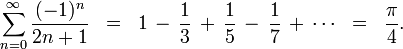
\includegraphics[width = 0.5\textwidth]{resources/Pi.png}
\end{center}
\end{frame}

\begin{frame}[fragile]{Actors by example}
\begin{exampleblock}{Dependency (not required since Scala 2.10)}
\begin{lstlisting}[basicstyle=\scriptsize]
resolvers += "Typesafe Repository" at "http://repo.typesafe.com/typesafe/releases/"

libraryDependencies += "com.typesafe.akka" % "akka-actor" % "2.0.2"
\end{lstlisting}
\end{exampleblock}
\pause
\begin{exampleblock}{Imports}
\begin{lstlisting}
import akka.actor._
import akka.routing.RoundRobinRouter
import akka.util.Duration
import akka.util.duration._
\end{lstlisting}
\end{exampleblock}
\end{frame}

\begin{frame}[fragile]{Actors by example}
\begin{lstlisting}
object Pi extends App {
  val system = ActorSystem("PiSystem")
  val listener = system.actorOf(Props[Listener], name = "listener")
  val master = system.actorOf(Props(new Master(
    nrOfWorkers = 4,
    nrOfMessages = 10000,
    nrOfElements = 10000,
    listener)), name = "master")
 
  master ! Calculate
}
\end{lstlisting}
\end{frame}

\begin{frame}[fragile]{Actors by example}
\begin{exampleblock}{Messages ADT}
\begin{lstlisting}
sealed trait PiMessage
case object Calculate extends PiMessage
case class Work(start: Int, nrOfElements: Int) extends PiMessage
case class Result(value: Double) extends PiMessage
case class PiApproximation(pi: Double, duration: Duration)
\end{lstlisting}
\end{exampleblock}
\end{frame}

\begin{frame}[fragile]{Actors by example}
\begin{exampleblock}{The Worker}
\onslide<1->
\begin{lstlisting}
class Worker extends Actor {
  def receive = {
    case Work(start, nrOfElements) =>
      sender ! Result(calculatePiFor(start, nrOfElements))
  }
\end{lstlisting}
\onslide<2->
\begin{lstlisting}
  def calculatePiFor(start: Int, nrOfElements: Int): Double = {
    var acc = 0.0
      for (n <- start until (start + nrOfElements))
        acc += 4.0 * (1 - (n % 2) * 2) / (2 * n + 1)
    acc
  }
\end{lstlisting}
\onslide<1->
\begin{lstlisting}
}
\end{lstlisting}
\end{exampleblock}
\end{frame}

\begin{frame}[fragile]{Actors by example}
\begin{exampleblock}{The Master}
\begin{lstlisting}
class Master(
  nrOfWorkers: Int,
  nrOfMessages: Int,
  nrOfElements: Int,
  listener: ActorRef) extends Actor {
  var pi: Double = _
  var nrOfResults: Int = _
  val start: Long = System.currentTimeMillis
     
  val workerRouter = context.actorOf(
    Props[Worker].withRouter(RoundRobinRouter(nrOfWorkers)),
    name = "workerRouter")
     
  def receive = {
    // handle messages ...
  } 
}
\end{lstlisting}
\end{exampleblock}
\end{frame}

\begin{frame}[fragile]{Actors by example}
\begin{exampleblock}{The Master}
\begin{lstlisting}
class Master(...) extends Actor {
  def receive = {
    case Calculate => for (i <- 0 until nrOfMessages)
      workerRouter ! Work(i * nrOfElements, nrOfElements)
    case Result(value) =>
      pi += value
      nrOfResults += 1
      if (nrOfResults == nrOfMessages) {
        listener ! PiApproximation(
          pi,
          (System.currentTimeMillis - start).millis
        )
        context.stop(self)
      }
  }
}
\end{lstlisting}
\end{exampleblock}
\end{frame}

\begin{frame}[fragile]{Actors by example}
\begin{exampleblock}{The Listener}
\begin{lstlisting}
class Listener extends Actor {
  def receive = {
    case PiApproximation(pi, duration) =>
      println("Pi approximation:%s\nCalculation time:%s"
      .format(pi, duration))
    context.system.shutdown()
  }
}
\end{lstlisting}
\end{exampleblock}
\end{frame}

\section{Summary}
\begin{frame}{Summary}
\begin{itemize}
  \item The \alert{single-threaded} world is coming to an end
  \item The future of computing lies in \highlight{concurrency}
  \item Concurrency is very very \alert{hard}
  \item \alert{Avoid} (shared) mutable state as much as you can
  \item Akka is a very powerful \highlight{state of the art} concurrency toolkit
  \item \highlight{Futures} and \highlight{Promises} are very useful abstractions for concurrency
  \item Actors are great for \highlight{distributed computing}
\end{itemize}
\end{frame}